\chapter*{Introduction} \label{intro}
As time goes by, we come to the conclusion that wildfires are 
some of the most fierce and dangerous threats to human and 
wildlife safety. \par
As reported by the Institute for Nature Conservation and Forests (ICNF), the
number of fire incidents in rural areas has exceeded 6,000 since the beginning of
this year (2024), with a total area of over 137,000 hectares affected by fire. \par 
\begin{figure}[H] 
\centering
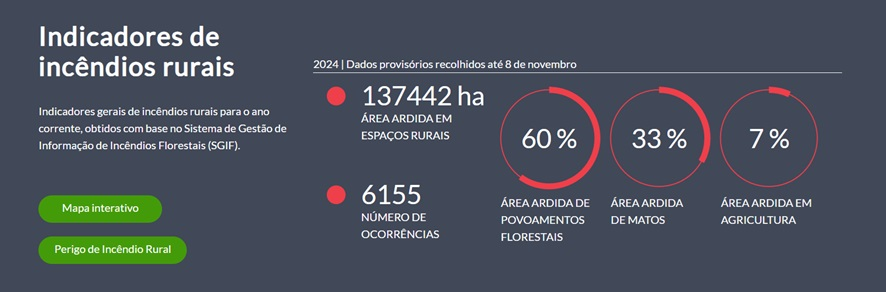
\includegraphics[width=\textwidth]{IndicadoresIncendiosICNF.jpg}
\caption{ICNF rural fire indicators}
\end{figure}
One of the ways to prevent wildfires is by using 
technological tools that can detect and combat them more 
effectively. \par 
The project is comprised of several stages, which have been classified into 
the following four
sections: 
\begin{itemize}
    \item Section 1: from the problem description to the 
    definition of stakeholders;
    \item Section 2: from the designed sketches to the iteration 
    process; 
    \item Section 3: from the description of the sketches in 
    low fidelity to a description
    of the constituent parts of the requested system for this project;
    \item Section 4: from aspects of human interaction with the system to the overall
    improvements made.
\end{itemize}


